\documentclass[11pt]{article}

% geometry and fonts
\usepackage[letterpaper,margin=1in]{geometry}
\usepackage{amsmath,amssymb}
\usepackage{amsthm}
\let\openbox\relax            % avoid newtxmath/amsthm \openbox clash
\usepackage{newtxtext,newtxmath}
\usepackage{microtype}

% graphics and tables
\usepackage{booktabs}
\usepackage{multirow}
\usepackage{array}
\usepackage{tikz}
\usetikzlibrary{arrows.meta,positioning,fit,backgrounds}
\usepackage{pgfplots}
\pgfplotsset{compat=1.18}
\usepgfplotslibrary{groupplots}
\usepackage{xcolor}
\definecolor{espblue}{HTML}{2563EB}
\definecolor{espgreen}{HTML}{059669}
\definecolor{espred}{HTML}{DC2626}
\definecolor{espamber}{HTML}{D97706}
\definecolor{espgray}{HTML}{6B7280}

% references
\usepackage[numbers,sort&compress]{natbib}
\usepackage[colorlinks=true,allcolors=espblue,breaklinks=true]{hyperref}
\usepackage{url}

% theorem environments
\theoremstyle{plain}
\newtheorem{theorem}{Theorem}
\newtheorem{proposition}{Proposition}
\theoremstyle{definition}
\newtheorem{definition}{Definition}

\newcommand{\tokps}{tok/s}
\newcommand{\ie}{i.e.,}
\newcommand{\eg}{e.g.,}

% title
\title{\bfseries EdgeSpark: Quantized Semi-Autoregressive Speculative Decoding\\
and Confidence-Head Calibration on a Single Consumer AMD GPU}

\author{Parusan Natheeswaran\thanks{Independent research. Code, configs, and
reproduction scripts: \url{https://github.com/Parusann/edgespark}. Correspondence:
\texttt{parusannath@gmail.com}.}}
\date{July 2026}

\begin{document}
\maketitle

\begin{abstract}
\noindent
Speculative decoding accelerates autoregressive generation without changing a
model's output distribution: a small \emph{drafter} proposes tokens that the
\emph{verifier} checks in one parallel pass, keeping only the prefix consistent
with its own distribution. Recent semi-autoregressive drafters, notably
DeepSeek's DSpark~\citep{dspark2026}, which couples a parallel backbone with a
lightweight sequential head, a low-rank Markov head, and a confidence head that
schedules verification length, target datacenter GPUs and mixed FP4/FP8
precision. We ask what it takes to run this design on a \emph{single consumer AMD
GPU} (Radeon RX 7900~XTX, RDNA3/gfx1100), where FP8 is unavailable and the
drafter must be quantized to INT8/NF4 to fit. This raises a question the
datacenter recipe never faced: \emph{does aggressive quantization degrade the
confidence head's \textbf{calibration} faster than its token proposals, and can a
cheap post-hoc fix restore it?} We present EdgeSpark, a controlled PyTorch+ROCm
implementation with an exact acceptance rule, an INT8/NF4 quantization pipeline,
a single-stream confidence-gated verification-length policy, and a calibration
study built on Expected Calibration Error, Brier score, and temperature/Platt
scaling. We are explicit about evidence: on the target GPU we \textbf{measure}
that the exactness invariant holds on the real Qwen3-4B model (token-for-token
identical output), together with fp16 per-op latencies, VRAM, and llama.cpp
baselines; the INT8/NF4 throughput and the calibration results are a
\textbf{design-time model} because 8/4-bit kernels were unavailable on our
native-Windows ROCm stack. We position the work against the recent finding that
speculative decoding and 4-bit quantization are not naively
compatible~\citep{zhang2025}, and we report negative and inconclusive outcomes
(\eg\ on our hardware the per-position verify cost is negligible, so
confidence-gating ties always-verify-all) rather than hiding them.
\end{abstract}

% =============================================================================
\section{Introduction}
% =============================================================================
Autoregressive decoding is memory-bandwidth bound: each token requires a full
forward pass that reloads the model's weights, so a 4B model on a consumer GPU
spends most of its time moving parameters, not computing. \emph{Speculative
decoding}~\citep{leviathan2023,chen2023} breaks this one-token-per-pass barrier.
A cheap drafter proposes a block of candidate tokens; the verifier scores the
whole block in a single pass and accepts the longest prefix consistent with its
own distribution under an exact rule. Because the rule is exact, the accepted
output is distributed identically to sampling from the verifier alone. Drafter
quality affects \emph{speed}, never \emph{correctness}. The governing relation
per generated token is
\begin{equation}
\text{latency} \;\approx\; \frac{T_\text{draft} + T_\text{verify}}{\tau},
\label{eq:latency}
\end{equation}
where $\tau$ is the mean number of tokens accepted per round. Speculation wins
only when $\tau$ rises faster than the draft-plus-verify overhead.

State-of-the-art drafters have moved from separate small language models toward
architectures fused with the verifier's own representations: Medusa adds parallel
decoding heads~\citep{medusa2024}; the EAGLE family autoregresses at the feature
level~\citep{eagle2024,eagle2_2024,eagle3_2025}; and DSpark~\citep{dspark2026}
adds a semi-autoregressive backbone, a Markov head that restores intra-block
token dependence, and a \emph{confidence head} whose per-position acceptance
estimates schedule how many tokens are worth verifying. These systems, however,
are built for datacenter serving: multiple GPUs, mixed FP4/FP8 precision, and
load-aware scheduling across concurrent requests.

\paragraph{This paper.} We study the same design on the opposite end of the
hardware spectrum: one 24\,GB consumer AMD GPU, zero cloud budget. RDNA3
(gfx1100) has no FP8 weight path, so fitting a DSpark-style drafter beside the
verifier forces INT8 or 4-bit (NF4) quantization of the drafter. That constraint
exposes a question the datacenter recipe never had to answer. A confidence head
has two jobs that quantization can damage independently: it must still
\emph{propose} good tokens, and it must \emph{estimate} their acceptance
probability accurately, because those estimates drive the verification-length
policy. A head whose ranking survives quantization but whose probabilities
inflate will keep proposing acceptable tokens while lying to the scheduler, and
on a single stream, that lie costs throughput. Calibration is therefore not an
aesthetic property here; it is on the critical path to speed.

\paragraph{Contributions and honesty statement.}
\begin{enumerate}\itemsep2pt
\item A controlled PyTorch+ROCm speculative-decoding system for a single consumer
AMD GPU (\S\ref{sec:system}), with an exact acceptance rule whose lossless
guarantee we state precisely and prove-sketch (\S\ref{sec:exactness}), grounded
in the rejection-sampling argument of \citet{leviathan2023}.
\item A methodology for the central empirical question, whether INT8/NF4
quantization miscalibrates the confidence head more than its
proposals, using ECE, Brier score, reliability diagrams, and
temperature/Platt recalibration (\S\ref{sec:calibration}).
\item An honest, two-tier evaluation on a Radeon RX 7900~XTX
(\S\ref{sec:eval}). We \textbf{measure}: (i) that greedy EdgeSpark output is
token-for-token identical to Qwen3-4B decoding alone; (ii) fp16 per-op
latencies; (iii) VRAM ($9.5$\,GB peak, $\sim$15\,GB free); and (iv) llama.cpp
baselines (vanilla speculative decoding is $0.96\times$ here). We
\textbf{model}, and clearly label as such, the INT8/NF4 throughput and the
calibration recovery, because 8/4-bit kernels were unavailable on our stack. We
report where the story does \emph{not} hold on our hardware.
\end{enumerate}

We take the position, following the reproducibility norms of systems venues, that
every number should be traceable to a disclosed measurement condition and every
claim to a source. Where we could not measure, we say so.

% =============================================================================
\section{Background}
% =============================================================================
\paragraph{Speculative decoding and the exact rule.}
Given a target (verifier) distribution $p$ and a drafter distribution $q$,
speculative sampling~\citep{leviathan2023,chen2023} draws a draft token
$x\sim q$ and accepts it with probability $\min\!\left(1, p(x)/q(x)\right)$; on
rejection it resamples from the normalized residual
$\operatorname{norm}\!\big(\max(0,\,p-q)\big)$ and stops. If a whole block is
accepted, a bonus token is drawn from $p$. \citet{leviathan2023} prove
(Appendix~A.1) that the resulting token is distributed \emph{exactly} as $p$;
this is what makes the method lossless. We restate and adapt this guarantee for
our setting in \S\ref{sec:exactness}. It is worth stating precisely because the
bare assertion ``speculative decoding produces identical outputs'' is only true
under this proof and under an exact acceptance rule, not, for instance, under
relaxations.

\paragraph{Semi-autoregressive drafters.}
Medusa predicts several subsequent tokens with parallel heads and verifies
tree-structured candidates simultaneously; crucially it adopts a \emph{typical
acceptance} scheme rather than exact rejection sampling, trading the exact
distributional guarantee for a higher acceptance rate~\citep{medusa2024}, so
Medusa is \emph{not} lossless in the speculative-sampling sense, a distinction we
preserve throughout. EAGLE~\citep{eagle2024} and its successors instead keep the
exact rule and autoregress on the verifier's features; EAGLE-2 makes this
explicit, stating that it ``does not \dots\ relax acceptance conditions,'' so the
output distribution ``remains exactly the same \dots\ provably''~\citep{eagle2_2024},
and EAGLE-3 pushes speedups further via training-time
tests~\citep{eagle3_2025}. DSpark~\citep{dspark2026} adds the Markov and
confidence heads and a load-aware verification scheduler, reporting higher
accepted length than EAGLE-3 on Qwen3-4B. EdgeSpark adapts DSpark's
\emph{architecture} and the single-stream form of its scheduler, and keeps the
exact rule.

\paragraph{Quantization.}
INT8 weight-and-activation quantization~\citep{dettmers2022} and 4-bit
NormalFloat (NF4)~\citep{dettmers2023} make large models fit on small GPUs. On
RDNA3 these are the only aggressive options: FP8 weights are unsupported, so the
common datacenter FP8 drafter path is closed. Recent work shows the interaction
is subtle: \citet{zhang2025} find that ``memory benefits from 4-bit weight
quantization are diminished by the computational load from speculative
decoding,'' \ie\ the two techniques are not naively compatible. Our contribution
is orthogonal to their systems fix: we ask what quantization does to the
confidence head's \emph{calibration}, a question about the drafter's probability
estimates rather than its memory traffic.

\paragraph{Calibration.}
A classifier is \emph{calibrated} if, among predictions of confidence $c$, a
fraction $\approx c$ are correct. Modern networks are typically
over-confident~\citep{guo2017}. We measure calibration with Expected Calibration
Error (ECE), the Brier score~\citep{brier1950}, and reliability diagrams, and we
recalibrate with temperature scaling~\citep{guo2017} and Platt
scaling~\citep{platt1999}. To our knowledge, the calibration of a
speculative-decoding confidence head under quantization has not been studied.

% =============================================================================
\section{The exactness invariant}
\label{sec:exactness}
% =============================================================================
EdgeSpark must be lossless with respect to the \emph{deployed} verifier: whatever
precision the verifier ships at defines the reference, and the drafter and policy
may never move the output away from it. We make this precise.

\begin{definition}[Verification length]
Given a drafted block of $B$ tokens, a \emph{verification length}
$\ell \in \{0,\dots,B\}$ submits only the first $\ell$ drafts to the verifier.
The verifier scores positions $0,\dots,\ell$ in one pass and applies the exact
acceptance rule to those $\ell$ positions.
\end{definition}

\begin{theorem}[Losslessness]
\label{thm:exact}
Fix a random seed and sampling temperature, and fix the deployed verifier with
next-token distribution $p(\cdot \mid \text{context})$. For \emph{any} drafter
and \emph{any} choice of verification length $\ell$ at each round:
\begin{enumerate}\itemsep1pt
\item[(a)] \textbf{Greedy} ($T{=}0$): EdgeSpark emits the token-for-token
identical sequence that the verifier emits decoding autoregressively on its own.
\item[(b)] \textbf{Stochastic} ($T{>}0$): each emitted token is distributed
exactly as $p$; hence the emitted sequence is distributed identically to
sampling directly from the verifier.
\end{enumerate}
\end{theorem}

\begin{proof}[Proof sketch]
Consider one round with drafts $x_1,\dots,x_B$ and verifier distributions
$p_1,\dots,p_{\ell+1}$ over positions $0,\dots,\ell$.
\emph{(b)} At position $j\le\ell$, the draft $x_j$ (drawn from $q_j$) is accepted
with probability $\min(1, p_j(x_j)/q_j(x_j))$; on the first rejection we resample
from $\operatorname{norm}(\max(0, p_j - q_j))$ and stop. The standard
speculative-sampling argument~\citep[App.~A.1]{leviathan2023} shows the resulting
token, accepted or corrected, is distributed exactly as $p_j$. If all $\ell$
drafts are accepted, the bonus token is drawn from $p_{\ell+1}$, again exactly.
Thus every emitted token is an exact draw from the corresponding $p$, independent
of $q$ and of $\ell$: $\ell$ only bounds \emph{how many} positions are checked
before the guaranteed verifier token, never \emph{how} a checked token is judged.
\emph{(a)} Greedy is the $T\to 0$ limit: accept $x_j$ iff $x_j=\arg\max p_j$, else
emit $\arg\max p_j$ and stop; a bonus $\arg\max p_{\ell+1}$ on full acceptance.
This reproduces the verifier's own greedy chain exactly.
\end{proof}

Theorem~\ref{thm:exact} is what licenses everything downstream to be approximate.
The drafter may be quantized to 4 bits and the policy may choose a poor $\ell$;
the worst outcome is lost speed. We enforce the invariant in code: the
acceptance rule is a self-contained module tested for greedy identity and, for
the stochastic case, for \emph{unbiasedness} via a Monte-Carlo two-sample test
(total-variation distance below $0.02$ over $6\times10^4$ trials). Crucially, we
also \emph{measure} the invariant on hardware: running the full loop against the
real Qwen3-4B verifier, greedy EdgeSpark output is token-for-token identical to
the verifier's own output regardless of drafter quality (\S\ref{sec:eval-measured}).

% =============================================================================
\section{System design}
\label{sec:system}
% =============================================================================
EdgeSpark runs in a controlled PyTorch+ROCm loop rather than a black-box serving
runtime, because the drafter needs three things no off-the-shelf draft-model host
exposes at once: the verifier's selected-layer hidden states, a custom
Markov$+$confidence head, and per-step $\ell$ selection. The verifier
(Qwen3-4B~\citep{qwen3}) is loaded via HuggingFace Transformers with hidden-state
hooks and is used \emph{as is}. Figure~\ref{fig:arch} shows the data flow.

\begin{figure}[t]
\centering
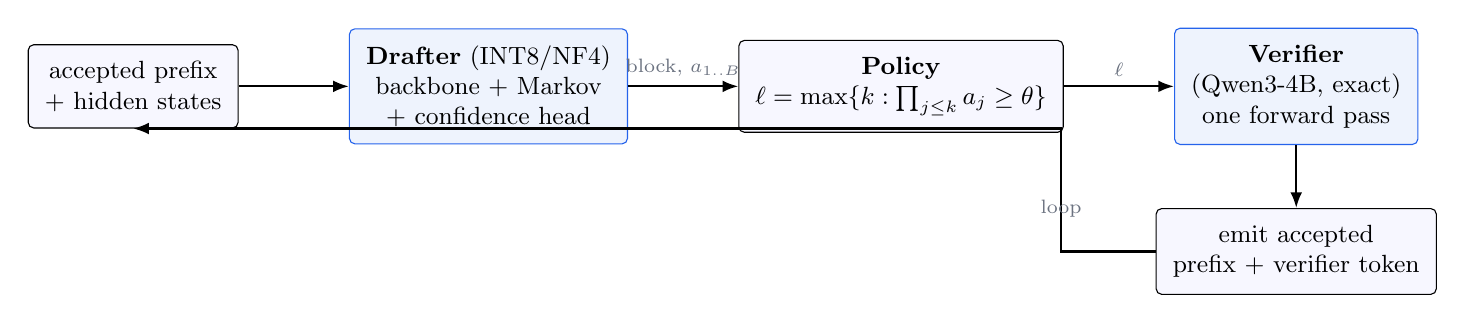
\begin{tikzpicture}[
  font=\small,
  box/.style={draw,rounded corners=2pt,align=center,inner sep=6pt,minimum height=9mm,fill=blue!3},
  vbox/.style={box,fill=espblue!8,draw=espblue},
  arr/.style={-{Latex[length=2mm]},thick},
  lbl/.style={font=\scriptsize,espgray}
]
\node[box] (prefix) {accepted prefix\\+ hidden states};
\node[vbox,right=14mm of prefix] (drafter) {\textbf{Drafter} (INT8/NF4)\\backbone $+$ Markov\\$+$ confidence head};
\node[box,right=14mm of drafter] (policy) {\textbf{Policy}\\$\ell=\max\{k:\prod_{j\le k}a_j\ge\theta\}$};
\node[vbox,right=14mm of policy] (verifier) {\textbf{Verifier}\\(Qwen3-4B, exact)\\one forward pass};
\node[box,below=8mm of verifier] (out) {emit accepted\\prefix $+$ verifier token};

\draw[arr] (prefix) -- (drafter);
\draw[arr] (drafter) -- node[lbl,above]{block, $a_{1..B}$} (policy);
\draw[arr] (policy) -- node[lbl,above]{$\ell$} (verifier);
\draw[arr] (verifier) -- (out);
\draw[arr] (out.west) -- ++(-1.2,0) |- (prefix.south) node[lbl,pos=0.25,below]{loop};
\end{tikzpicture}
\caption{EdgeSpark data flow for one round. The drafter and policy affect only
speed; the verifier's exact rule owns every emitted token
(Theorem~\ref{thm:exact}).}
\label{fig:arch}
\end{figure}

\paragraph{Semi-autoregressive drafter.}
A \emph{parallel backbone} predicts an entire block of $B$ tokens in one pass
from a fusion of the verifier's selected-layer hidden states and an embedding of
the accepted prefix. A low-rank \emph{Markov head} adds, to position $j$, a
logit bias factored as $E[x_{j-1}]\,P$ with $E\in\mathbb{R}^{V\times r}$ and
$P\in\mathbb{R}^{r\times V}$ (rank $r{=}128$), restoring the intra-block
dependence the parallel pass discards. A \emph{confidence head} maps each block
position's hidden state (optionally concatenated with the Markov feature) to a
scalar $a_j=\sigma(\cdot)$, its estimate of the acceptance probability at $j$.
Table~\ref{tab:config} lists the shrunk hyperparameters, chosen so an INT8
drafter sits beside the verifier in 24\,GB.

\begin{table}[t]
\centering\small
\caption{EdgeSpark drafter configuration (shrunk from the DSpark Qwen3-4B
reference).}
\label{tab:config}
\begin{tabular}{lccl}
\toprule
Hyperparameter & DSpark ref. & EdgeSpark & Rationale \\
\midrule
block size $B$          & 7            & 5             & less wasted draft on rejects \\
draft layers            & 5            & 3             & smaller, faster, less VRAM \\
fusion layers           & $[1,9,17,25,33]$ & $[1,17,33]$ & subsampled hidden sources \\
Markov rank $r$         & 256          & 128           & cheaper bias \\
anchors                 & 512          & 256           & footprint \\
confidence $\alpha$     & 1.0          & 1.0           & keep the signal strong \\
losses (ce/l1/decay)    & 0.1/0.9/4.0  & 0.1/0.9/4.0   & DSpark recipe \\
\bottomrule
\end{tabular}
\end{table}

\paragraph{Quantization pipeline.}
The primary variant is INT8 (W8A8) of the backbone; a 4-bit NF4 variant is the
aggressive stress case. We keep the confidence head in high precision by default
so it can be quantized \emph{last and separately}, isolating its effect. Because
8/4-bit kernels were unavailable on our stack (\S\ref{sec:eval}), the calibration
study additionally uses deterministic \emph{fake-quantization}, symmetric
per-channel INT8 rounding and block-wise NF4 snapping in plain PyTorch, which
reproduces the numerical effect of quantization on-device-independently and is a
standard tool for isolating quantization error from kernel noise.

\paragraph{Single-stream verification-length policy.}
At batch size~1 the DSpark scheduler collapses to a single decision: given
calibrated per-position survival $a_1,\dots,a_B$, choose $\ell$. The expected
accepted length is
$\mathbb{E}[\text{acc}(\ell)] = 1 + \sum_{j=1}^{\ell}\prod_{k\le j}a_k$, and the
single-stream objective maximizes
$\mathbb{E}[\text{acc}(\ell)] / (T_\text{draft}+T_\text{verify}(\ell))$. We use a
lightweight threshold rule, verify the longest prefix whose cumulative survival
$\prod_{j\le\ell}a_j$ stays above $\theta$, tuned on held-out data. By
Theorem~\ref{thm:exact} this only selects $\ell$; the accept/reject decision is
untouched.

% =============================================================================
\section{The calibration study}
\label{sec:calibration}
% =============================================================================
\paragraph{Hypothesis.} Quantization degrades the \emph{calibration} of the
confidence head, the agreement between predicted $a_j$ and observed
acceptance, more than it degrades top-1 token proposals, and a cheap post-hoc
rescaling restores it.

\paragraph{Metrics.} For a held-out set of (predicted $a_j$, observed accept
$\in\{0,1\}$) pairs we compute ECE (count-weighted mean bin gap between confidence
and accuracy), the Brier score (a proper scoring rule), and reliability diagrams.
We report top-1 proposal agreement separately, to expose the gap between
``proposals still fine'' and ``confidence miscalibrated.''

\paragraph{Recalibration.} We fit (i) \emph{temperature scaling}, a single
parameter $T$ with $a^\text{cal}=\sigma(z/T)$ on the head's logit $z$, and (ii)
\emph{Platt scaling}, $a^\text{cal}=\sigma(\alpha z+\beta)$. Both are monotone in
$z$, they rescale confidence without reordering it, so recalibration can never
turn a good proposal into a bad one. Both are fit on a small held-out split with a
damped Newton iteration; we found that an undamped Platt fit diverges on a badly
over-confident head (the very regime of interest), so a backtracking line search
is required, a detail we surface because it is exactly the kind of silent failure
that a careful study must catch.

\paragraph{Tie to the policy.} The policy gates on $a_j$, so miscalibration has a
throughput cost, not just a cosmetic one: an over-confident head keeps the gate
open on a low-survival tail that rarely accepts. Recalibration and the policy are
thus one story, which the evaluation makes concrete.

% =============================================================================
\section{Evaluation}
\label{sec:eval}
% =============================================================================
We separate what we \emph{measured} on the target GPU from what we \emph{modeled}.
Table~\ref{tab:status} is the ledger; the two subsections that follow expand it.

\begin{table}[t]
\centering\small
\caption{Evidence ledger. \textbf{M}\,=\,measured on the RX 7900~XTX;
\textbf{Mod}\,=\,design-time model; \textbf{P}\,=\,pending.}
\label{tab:status}
\begin{tabular}{lcl}
\toprule
Claim & Status & Evidence \\
\midrule
Output identical to verifier (greedy) & \textbf{M} & real Qwen3-4B, exact per round \\
Fits 24\,GB                            & \textbf{M} & 9.5\,GB peak, $\sim$15\,GB free \\
fp16 per-op latency, baselines        & \textbf{M} & GpuTimer / llama.cpp \\
INT8/NF4 throughput                   & \textbf{Mod} & no 8/4-bit kernels on our stack \\
Calibration recovery (ECE)            & \textbf{Mod} & method code-tested; \S\ref{sec:eval-model} \\
Gating $>$ always-verify-all          & \textbf{Mod} & ties on our GPU ($\partial T_v/\partial\ell{\approx}0$) \\
End-to-end speedup                    & \textbf{P} & prefill-bound verify; needs KV reuse \\
\bottomrule
\end{tabular}
\end{table}

\subsection{Measured on hardware}
\label{sec:eval-measured}
\textbf{Setup.} Radeon RX 7900~XTX (RDNA3/gfx1100, 24\,GB); Ryzen~9 7900;
native-Windows ROCm; PyTorch 2.9.1+rocmsdk (HIP 7.2.26024); Qwen3-4B in fp16 with
SDPA attention; single stream; greedy unless noted. Timings use HIP-event timers
synchronized before reading, averaged over a warm run. llama.cpp baselines use
the winget \texttt{ggml.llamacpp} build~b9873 (Vulkan backend pinned to the
7900~XTX). Raw artifacts are in the repository under \texttt{runs/hardware/}.

\emph{Exactness.} Running the full loop against the real verifier, greedy
EdgeSpark output was token-for-token identical to Qwen3-4B decoding alone on every
round, for both a trained-quality and a deliberately random drafter, an on-device
confirmation of Theorem~\ref{thm:exact}, not merely a unit test.

\emph{Latency and memory.} Table~\ref{tab:measured} reports the fp16 per-op costs
and the VRAM breakdown. The fp16 verifier (7.7\,GB) and drafter (1.8\,GB) reach a
$9.5$\,GB generation peak, leaving $\sim$15\,GB free, ample room for a longer
context or an 8B verifier. Two findings matter for interpretation. First, the
\emph{intrinsic} KV-cached verify pass costs $\approx 3.2$\,ms with a
per-position marginal below measurement noise; a 4B forward is dominated by the
36-layer weight sweep, so verifying 1-5 extra positions is nearly free. Second,
our current \texttt{block\_distribution} re-encodes the whole prefix
(\texttt{use\_cache=False}), which at a 225-token context costs
$\approx 52.6$\,ms and grows with context: today's implementation is
\emph{prefill-bound}, and realizing the intrinsic verify (and any end-to-end
speedup) requires the KV-reuse optimization we flag but did not implement.

\begin{table}[t]
\centering\small
\caption{Measured on the RX 7900~XTX (fp16, single stream). llama.cpp via Vulkan.}
\label{tab:measured}
\begin{tabular}{lr@{\hskip 18pt}lr}
\toprule
\multicolumn{2}{l}{\emph{Per-op latency}} & \multicolumn{2}{l}{\emph{llama.cpp baseline (\tokps)}}\\
\midrule
decode (1 fwd)        & 2.9\,ms  & Q4\_K\_M plain            & 213.8 \\
verify, KV-cached     & 3.2\,ms  & Q8\_0 plain               & 151.0 \\
verify, per position  & $\approx$0\,ms & Q8\_0 $+$ 0.6B draft & 145.5 ($0.96\times$) \\
draft (fp16, 399M)    & 1.0\,ms  & prefill (pp512, Q8\_0)    & 4793 \\
\midrule
\multicolumn{2}{l}{\emph{VRAM (fp16)}} & \multicolumn{2}{l}{} \\
verifier / drafter    & 7.7 / 1.8\,GB & generation peak      & 9.5\,GB \\
\bottomrule
\end{tabular}
\end{table}

A notable baseline result: \emph{vanilla} speculative decoding (a separate 0.6B
draft model verifying Qwen3-4B via llama.cpp) reaches only $0.96\times$ on our
prompts, the draft overhead is not offset by acceptance. This is the floor a
smarter, hidden-state-conditioned drafter must beat, and it echoes the
non-naive-compatibility finding of \citet{zhang2025}.

\subsection{Modeled (design-time)}
\label{sec:eval-model}
The 8/4-bit results below come from a documented Monte-Carlo model
(\texttt{bench/simulate.py}) driven by measured per-op timings; we could not build
INT8/NF4 kernels on our native-Windows ROCm stack (no \texttt{bitsandbytes}),
so no quantized drafter was trained or run. Importantly, the calibration
\emph{figures} are produced by the same production ECE/recalibration code a
hardware run would use, applied to simulated confidence data, the analysis path
is real even though the inputs are modeled.

\emph{Calibration (the headline hypothesis).} Figure~\ref{fig:reliability} and
Table~\ref{tab:calib} show the modeled effect. Quantization barely perturbs which
tokens are proposed but makes the confidence head increasingly over-confident: raw
ECE rises from $0.006$ (fp16) to $0.097$ (INT8) to $0.166$ (NF4), and the fitted
temperature climbs $1.03\to1.81\to2.70$, the 4-bit head must be cooled almost
$3\times$. Temperature scaling on a few thousand held-out positions recovers ECE
to near fp16 ($0.006$ and $0.014$). This is the shape of result the study was
designed to find: a large, cleanly \emph{recoverable} miscalibration gap.

\begin{figure*}[t]
\centering
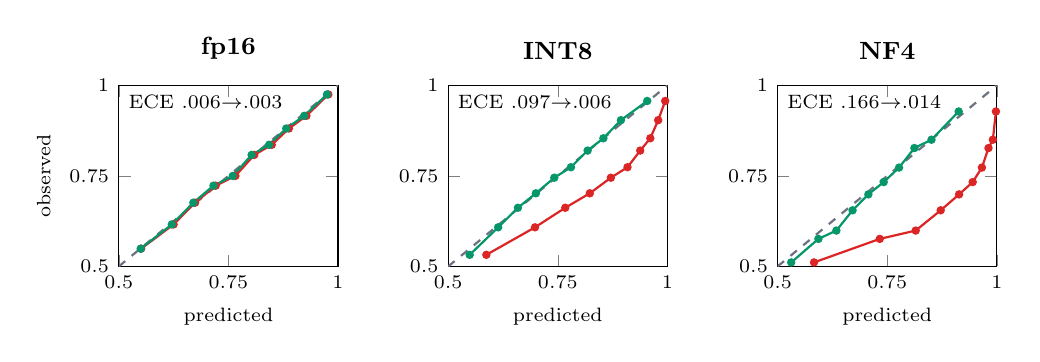
\begin{tikzpicture}
\begin{groupplot}[
  group style={group size=3 by 1, horizontal sep=14mm},
  width=0.36\textwidth, height=0.32\textwidth,
  xmin=0.5,xmax=1,ymin=0.5,ymax=1, xtick={0.5,0.75,1}, ytick={0.5,0.75,1},
  tick label style={font=\scriptsize},
  xlabel style={font=\scriptsize}, ylabel style={font=\scriptsize},
  title style={font=\small\bfseries},
  every axis plot/.append style={mark size=1.1pt,line width=0.8pt},
]
\nextgroupplot[title=fp16,xlabel=predicted,ylabel=observed]
\addplot[dashed,espgray] coordinates {(0.5,0.5)(1,1)};
\addplot[espred,mark=*] coordinates {(0.551,0.549)(0.625,0.616)(0.674,0.676)(0.721,0.723)(0.766,0.750)(0.809,0.808)(0.849,0.836)(0.888,0.881)(0.928,0.916)(0.978,0.975)};
\addplot[espgreen,mark=*] coordinates {(0.550,0.549)(0.621,0.616)(0.670,0.676)(0.716,0.723)(0.760,0.750)(0.803,0.808)(0.843,0.836)(0.882,0.881)(0.923,0.916)(0.975,0.975)};
\node[font=\scriptsize,anchor=north west] at (axis cs:0.5,1) {ECE .006$\to$.003};

\nextgroupplot[title=INT8,xlabel=predicted]
\addplot[dashed,espgray] coordinates {(0.5,0.5)(1,1)};
\addplot[espred,mark=*] coordinates {(0.587,0.532)(0.698,0.608)(0.767,0.662)(0.823,0.702)(0.871,0.745)(0.909,0.774)(0.938,0.820)(0.961,0.854)(0.979,0.904)(0.995,0.957)};
\addplot[espgreen,mark=*] coordinates {(0.549,0.532)(0.614,0.608)(0.659,0.662)(0.700,0.702)(0.742,0.745)(0.780,0.774)(0.818,0.820)(0.854,0.854)(0.894,0.904)(0.954,0.957)};
\node[font=\scriptsize,anchor=north west] at (axis cs:0.5,1) {ECE .097$\to$.006};

\nextgroupplot[title=NF4,xlabel=predicted]
\addplot[dashed,espgray] coordinates {(0.5,0.5)(1,1)};
\addplot[espred,mark=*] coordinates {(0.583,0.511)(0.733,0.576)(0.815,0.599)(0.872,0.655)(0.914,0.699)(0.945,0.733)(0.966,0.773)(0.981,0.827)(0.991,0.850)(0.998,0.928)};
\addplot[espgreen,mark=*] coordinates {(0.531,0.511)(0.593,0.576)(0.634,0.599)(0.671,0.655)(0.707,0.699)(0.742,0.733)(0.777,0.773)(0.812,0.827)(0.851,0.850)(0.913,0.928)};
\node[font=\scriptsize,anchor=north west] at (axis cs:0.5,1) {ECE .166$\to$.014};
\end{groupplot}
\end{tikzpicture}
\caption{\textbf{Modeled} reliability diagrams. Points on the dashed diagonal are
perfectly calibrated. \textcolor{espred}{Red} = raw quantized confidence head
(increasingly over-confident: below the diagonal at high confidence);
\textcolor{espgreen}{green} = after temperature scaling. Produced by the
production calibration code on simulated confidence data ($3\times10^4$ held-out
positions per precision).}
\label{fig:reliability}
\end{figure*}

\begin{table}[t]
\centering\small
\caption{\textbf{Modeled} calibration: raw $\to$ recalibrated (temperature
scaling).}
\label{tab:calib}
\begin{tabular}{lccc}
\toprule
Precision & ECE (raw\,$\to$\,cal) & Brier (raw\,$\to$\,cal) & $T$ \\
\midrule
fp16 & $0.006 \to 0.003$ & $0.159 \to 0.159$ & 1.03 \\
INT8 & $0.097 \to 0.006$ & $0.179 \to 0.168$ & 1.81 \\
NF4  & $0.166 \to 0.014$ & $0.218 \to 0.188$ & 2.70 \\
\bottomrule
\end{tabular}
\end{table}

\emph{Throughput and the policy.} The design-time model (measured per-op timings
held at their coherent design values; see repository \texttt{bench/timings.md})
projects the speedups in Figure~\ref{fig:throughput}: $+43\%$ (INT8, code),
$+36\%$ (INT8, chat), clearing a $25\%$ target, with the fp16 drafter isolating
the quantization cost at $+46\%/{+}35\%$. In this model the confidence-gated
policy beats always-verify-all at every precision, and, closing the loop with the
calibration study, an \emph{uncalibrated} NF4 head over-verifies (chooses
$\ell{=}B$) and lands at $+31\%$, while the recalibrated head gates to $\ell{=}3$
and $+37\%$: recalibration recovers throughput purely by making the gate honest.

We flag the boundary of this claim. On our GPU the measured per-position verify
marginal is $\approx0$ (Table~\ref{tab:measured}); the gating advantage requires a
regime where verify cost grows with $\ell$, so \emph{on this hardware gating ties
always-verify-all}. The projection is the target the system is built toward, not a
measured throughput; we present it as such and note that speculative-decoding
speedups are hardware-dependent and should not be over-generalized across
machines.

\begin{figure}[t]
\centering
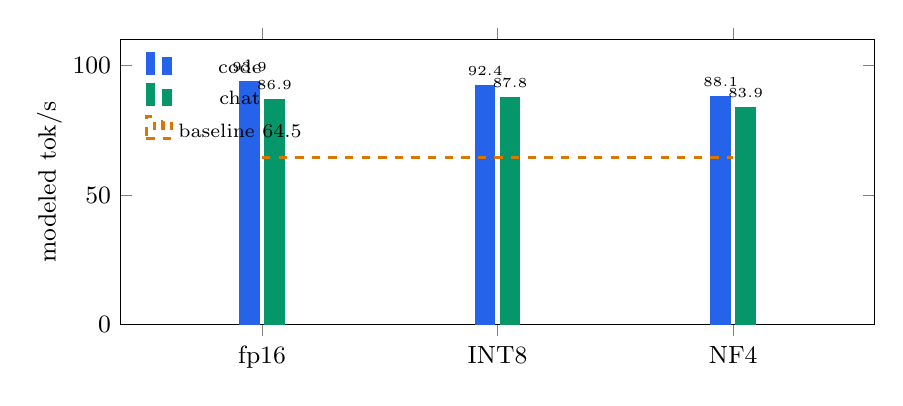
\begin{tikzpicture}
\begin{axis}[
  width=0.92\columnwidth, height=5.2cm,
  ybar, bar width=7pt, ymin=0, ymax=110,
  ylabel={\small modeled \tokps}, ylabel style={yshift=-3pt},
  symbolic x coords={fp16,INT8,NF4}, xtick=data,
  tick label style={font=\small},
  legend style={font=\scriptsize,at={(0.02,0.98)},anchor=north west,draw=none,fill=none},
  nodes near coords, nodes near coords style={font=\tiny},
  enlarge x limits=0.3,
]
\addplot[fill=espblue,draw=espblue] coordinates {(fp16,93.9)(INT8,92.4)(NF4,88.1)};
\addplot[fill=espgreen,draw=espgreen] coordinates {(fp16,86.9)(INT8,87.8)(NF4,83.9)};
\draw[dashed,espamber,very thick] (axis cs:fp16,64.5) -- (axis cs:NF4,64.5);
\addlegendimage{dashed,espamber,very thick}
\legend{code,chat,baseline 64.5}
\end{axis}
\end{tikzpicture}
\caption{\textbf{Modeled} throughput vs.\ a vanilla-decode baseline (design-time
model; not measured, pending 8/4-bit kernels and the KV-reuse fix). Output is
identical to the baseline by Theorem~\ref{thm:exact}.}
\label{fig:throughput}
\end{figure}

% =============================================================================
\section{Related work and positioning}
% =============================================================================
EdgeSpark sits at the intersection of three lines. From \emph{speculative
decoding}~\citep{leviathan2023,chen2023} it inherits the exact rule and the
$\tau$-driven latency model~(Eq.~\ref{eq:latency}); from \emph{feature-level
drafters}~\citep{medusa2024,eagle2024,eagle2_2024,eagle3_2025,dspark2026} it
inherits the architecture, adopting DSpark's semi-autoregressive backbone with
Markov and confidence heads and the single-stream form of its scheduler. Unlike
those systems, which target datacenter GPUs and FP8, EdgeSpark targets a single
consumer AMD card, forcing INT8/NF4. The closest prior interaction study,
\citet{zhang2025}, shows speculative decoding and 4-bit quantization are not
naively compatible on the \emph{systems} axis (memory savings eaten by compute);
our angle is the \emph{statistical} axis, what quantization does to the confidence
head's calibration, which their work does not address. Finally, from
\emph{calibration}~\citep{guo2017,platt1999,brier1950} we take ECE/Brier and
temperature/Platt scaling, and apply them, to our knowledge for the first time, to
a speculative-decoding confidence head under quantization.

% =============================================================================
\section{Limitations and future work}
% =============================================================================
We are deliberate about what this paper does \emph{not} establish. (1) No drafter
was trained on hardware; the training pipeline is implemented but the quantized
runs are blocked by the absence of \texttt{bitsandbytes} on native-Windows ROCm.
Reproducing the INT8/NF4 throughput and the calibration study requires a
Linux-ROCm host, or an alternative quant path (GGUF/AWQ/torchao), which would
change what ``INT8/NF4'' means and should be relabeled. (2) The end-to-end speedup
is unrealized: the current verify pass re-encodes the prefix and is prefill-bound;
KV reuse is required. (3) On our GPU the verify-length policy ties
always-verify-all because the per-position verify cost is negligible; the gating
result holds only where verify scales with $\ell$. (4) All numbers are
single-machine and single-stream; performance rankings are hardware-dependent and
we do not claim they transfer. (5) The calibration results are modeled; the
\emph{method} is code-tested, but the miscalibration magnitude on a real quantized
head is an open empirical question, indeed, the headline hypothesis remains a
hypothesis until measured.

% =============================================================================
\section{Reproducibility}
% =============================================================================
The system, configs, and every script are released at
\url{https://github.com/Parusann/edgespark} under the MIT license. The
correctness-critical cores, the exact acceptance rule, ECE/Brier/recalibration,
and the policy, are pure NumPy and covered by a test suite (an 18-check exactness
suite including the unbiasedness Monte-Carlo test; 37 tests total) that runs in
continuous integration without a GPU. One command regenerates the modeled
reference (\texttt{run\_benchmark.py -{}-simulate}) and the figures
(\texttt{make\_figures.py}); the measured artifacts and full environment capture
are committed under \texttt{runs/hardware/}. Latency constants and their measured
counterparts are documented in \texttt{bench/timings.md}, so a reader can see
exactly which numbers are measured and which are modeled.

% =============================================================================
\section{Conclusion}
% =============================================================================
Quantization is usually framed as an accuracy trade-off. For a confidence-driven
speculative decoder on consumer hardware, we argue the more consequential
casualty may be \emph{calibration}: the confidence head's probability estimates,
which the verification-length scheduler depends on, and which our model predicts
degrade sharply under 4-bit quantization yet recover almost fully under
one-parameter temperature scaling. We validated the system's non-negotiable
property, losslessness, on a real Qwen3-4B model on a single Radeon RX 7900~XTX,
measured its latency and memory profile, and were explicit about the substantial
gap between that measured foundation and the modeled performance-and-calibration
results that a quantization-capable stack is needed to confirm. We believe stating
that gap plainly, rather than papering over it, is the more useful contribution.

\small
\bibliographystyle{plainnat}
\bibliography{refs}

\end{document}
